\documentclass[12pt,a4paper]{article}
\usepackage{lmodern}
\usepackage{amssymb,amsmath}
\usepackage{ifxetex,ifluatex}
\usepackage{fixltx2e} % provides \textsubscript
\ifnum 0\ifxetex 1\fi\ifluatex 1\fi=0 % if pdftex
  \usepackage[T1]{fontenc}
  \usepackage[utf8]{inputenc}
\else % if luatex or xelatex
  \ifxetex
    \usepackage{mathspec}
  \else
    \usepackage{fontspec}
  \fi
  \defaultfontfeatures{Ligatures=TeX,Scale=MatchLowercase}
\fi
% use upquote if available, for straight quotes in verbatim environments
\IfFileExists{upquote.sty}{\usepackage{upquote}}{}
% use microtype if available
\IfFileExists{microtype.sty}{%
\usepackage{microtype}
\UseMicrotypeSet[protrusion]{basicmath} % disable protrusion for tt fonts
}{}
\usepackage[margin=1in]{geometry}
\usepackage{hyperref}
\hypersetup{unicode=true,
            pdftitle={Mastering GDAL Tools (Free Online Couse)},
            pdfauthor={Ujaval Gandhi},
            pdfborder={0 0 0},
            breaklinks=true}
\urlstyle{same}  % don't use monospace font for urls
\usepackage{color}
\usepackage{fancyvrb}
\newcommand{\VerbBar}{|}
\newcommand{\VERB}{\Verb[commandchars=\\\{\}]}
\DefineVerbatimEnvironment{Highlighting}{Verbatim}{commandchars=\\\{\}}
% Add ',fontsize=\small' for more characters per line
\usepackage{framed}
\definecolor{shadecolor}{RGB}{248,248,248}
\newenvironment{Shaded}{\begin{snugshade}}{\end{snugshade}}
\newcommand{\AlertTok}[1]{\textcolor[rgb]{0.94,0.16,0.16}{#1}}
\newcommand{\AnnotationTok}[1]{\textcolor[rgb]{0.56,0.35,0.01}{\textbf{\textit{#1}}}}
\newcommand{\AttributeTok}[1]{\textcolor[rgb]{0.77,0.63,0.00}{#1}}
\newcommand{\BaseNTok}[1]{\textcolor[rgb]{0.00,0.00,0.81}{#1}}
\newcommand{\BuiltInTok}[1]{#1}
\newcommand{\CharTok}[1]{\textcolor[rgb]{0.31,0.60,0.02}{#1}}
\newcommand{\CommentTok}[1]{\textcolor[rgb]{0.56,0.35,0.01}{\textit{#1}}}
\newcommand{\CommentVarTok}[1]{\textcolor[rgb]{0.56,0.35,0.01}{\textbf{\textit{#1}}}}
\newcommand{\ConstantTok}[1]{\textcolor[rgb]{0.00,0.00,0.00}{#1}}
\newcommand{\ControlFlowTok}[1]{\textcolor[rgb]{0.13,0.29,0.53}{\textbf{#1}}}
\newcommand{\DataTypeTok}[1]{\textcolor[rgb]{0.13,0.29,0.53}{#1}}
\newcommand{\DecValTok}[1]{\textcolor[rgb]{0.00,0.00,0.81}{#1}}
\newcommand{\DocumentationTok}[1]{\textcolor[rgb]{0.56,0.35,0.01}{\textbf{\textit{#1}}}}
\newcommand{\ErrorTok}[1]{\textcolor[rgb]{0.64,0.00,0.00}{\textbf{#1}}}
\newcommand{\ExtensionTok}[1]{#1}
\newcommand{\FloatTok}[1]{\textcolor[rgb]{0.00,0.00,0.81}{#1}}
\newcommand{\FunctionTok}[1]{\textcolor[rgb]{0.00,0.00,0.00}{#1}}
\newcommand{\ImportTok}[1]{#1}
\newcommand{\InformationTok}[1]{\textcolor[rgb]{0.56,0.35,0.01}{\textbf{\textit{#1}}}}
\newcommand{\KeywordTok}[1]{\textcolor[rgb]{0.13,0.29,0.53}{\textbf{#1}}}
\newcommand{\NormalTok}[1]{#1}
\newcommand{\OperatorTok}[1]{\textcolor[rgb]{0.81,0.36,0.00}{\textbf{#1}}}
\newcommand{\OtherTok}[1]{\textcolor[rgb]{0.56,0.35,0.01}{#1}}
\newcommand{\PreprocessorTok}[1]{\textcolor[rgb]{0.56,0.35,0.01}{\textit{#1}}}
\newcommand{\RegionMarkerTok}[1]{#1}
\newcommand{\SpecialCharTok}[1]{\textcolor[rgb]{0.00,0.00,0.00}{#1}}
\newcommand{\SpecialStringTok}[1]{\textcolor[rgb]{0.31,0.60,0.02}{#1}}
\newcommand{\StringTok}[1]{\textcolor[rgb]{0.31,0.60,0.02}{#1}}
\newcommand{\VariableTok}[1]{\textcolor[rgb]{0.00,0.00,0.00}{#1}}
\newcommand{\VerbatimStringTok}[1]{\textcolor[rgb]{0.31,0.60,0.02}{#1}}
\newcommand{\WarningTok}[1]{\textcolor[rgb]{0.56,0.35,0.01}{\textbf{\textit{#1}}}}
\usepackage{graphicx,grffile}
\makeatletter
\def\maxwidth{\ifdim\Gin@nat@width>\linewidth\linewidth\else\Gin@nat@width\fi}
\def\maxheight{\ifdim\Gin@nat@height>\textheight\textheight\else\Gin@nat@height\fi}
\makeatother
% Scale images if necessary, so that they will not overflow the page
% margins by default, and it is still possible to overwrite the defaults
% using explicit options in \includegraphics[width, height, ...]{}
\setkeys{Gin}{width=\maxwidth,height=\maxheight,keepaspectratio}
\IfFileExists{parskip.sty}{%
\usepackage{parskip}
}{% else
\setlength{\parindent}{0pt}
\setlength{\parskip}{6pt plus 2pt minus 1pt}
}
\setlength{\emergencystretch}{3em}  % prevent overfull lines
\providecommand{\tightlist}{%
  \setlength{\itemsep}{0pt}\setlength{\parskip}{0pt}}
\setcounter{secnumdepth}{0}
% Redefines (sub)paragraphs to behave more like sections
\ifx\paragraph\undefined\else
\let\oldparagraph\paragraph
\renewcommand{\paragraph}[1]{\oldparagraph{#1}\mbox{}}
\fi
\ifx\subparagraph\undefined\else
\let\oldsubparagraph\subparagraph
\renewcommand{\subparagraph}[1]{\oldsubparagraph{#1}\mbox{}}
\fi

%%% Use protect on footnotes to avoid problems with footnotes in titles
\let\rmarkdownfootnote\footnote%
\def\footnote{\protect\rmarkdownfootnote}

%%% Change title format to be more compact
\usepackage{titling}

% Create subtitle command for use in maketitle
\providecommand{\subtitle}[1]{
  \posttitle{
    \begin{center}\large#1\end{center}
    }
}

\setlength{\droptitle}{-2em}

  \title{Mastering GDAL Tools (Free Online Couse)}
    \pretitle{\vspace{\droptitle}\centering\huge}
  \posttitle{\par}
  \subtitle{Satellite and aerial image processing using GDAL tools}
  \author{Ujaval Gandhi}
    \preauthor{\centering\large\emph}
  \postauthor{\par}
    \date{}
    \predate{}\postdate{}
  
\usepackage{fancyhdr}
\pagestyle{fancy}
\renewcommand{\footrulewidth}{0.4pt}
\fancyhead[LE,RO]{\thepage}
\geometry{left=1in,top=0.75in,bottom=0.75in}
\fancyfoot[CE,CO]{{
\includegraphics[width=0.4cm]{images/gdal/cc.png}} {
\includegraphics[width=0.4cm]{images/gdal/by.png}} Ujaval Gandhi http://www.spatialthoughts.com}

\begin{document}
\maketitle

{
\setcounter{tocdepth}{3}
\tableofcontents
}
\newpage

This course is also offered as a in-person class. Please visit
\href{https://spatialthoughts.com}{www.spatialthoughts.com} to see the
schedule for upcoming sessions.

\newpage

\hypertarget{introduction}{%
\section{Introduction}\label{introduction}}

\href{https://gdal.org/}{GDAL} is an open-source library for raster and
vector geospatial data formats. The library comes with a vast collection
of utility programs that can perform many geoprocessing tasks. This
class introduces GDAL utilities with example workflows for processing
satellite and aerial imagery.

\hypertarget{get-the-data-package}{%
\section{Get the Data Package}\label{get-the-data-package}}

The code examples in this class use a variety of datasets. All the
required datasets are available in the
\href{http://bit.ly/gdal-tools-data}{gdal\_tools.zip}
{[}\textasciitilde1.3GB{]}. Download and unzip this file to the
\texttt{Downloads} directory. All commands below assume the data is
available in the
\texttt{\textless{}home\ folder\textgreater{}/Downloads/gdal\_tools/}
directory.

\hypertarget{running-gdal-commands}{%
\section{Running GDAL Commands}\label{running-gdal-commands}}

On Windows, the easiest way to run the gdal commands is via the
\textbf{OSGeo4W Shell}. To install GDAL commands, download the
\href{https://trac.osgeo.org/osgeo4w/}{OsGeo4W Installer} and run
Express Install. Once installed, launch the \emph{OsGeo4W Shell} and
\texttt{cd} to the \texttt{gdal\_tools} directory.

\begin{quote}
\begin{quote}
\textbf{Note:} Many commandline examples are long and span multiple
lines. To improve readability, they are separated by \textbf{\^{}}
character at the end if each line. This is a line continuation character
that enables the OsGeo4W shell to interpret it as a single command. If
you are running these on Mac or Linux, replace the \textbf{\^{}}
character with \textbf{\textbackslash{}}
\end{quote}
\end{quote}

\hypertarget{processing-satellite-data}{%
\section{Processing Satellite Data}\label{processing-satellite-data}}

This secsion shows how to take satellite data from Landsat-8 and create
various derived products.

\hypertarget{merging-individual-bands-into-rgb-composite}{%
\subsection{Merging individual bands into RGB
composite}\label{merging-individual-bands-into-rgb-composite}}

\begin{Shaded}
\begin{Highlighting}[]
\ExtensionTok{gdal_merge}\NormalTok{ -o rgb.tif -separate ^}
  \ExtensionTok{-co}\NormalTok{ PHOTOMETRIC=RGB -co COMPRESS=DEFLATE ^}
  \ExtensionTok{landsat8/RT_LC08_L1TP_137042_20190920_20190926_01_T1_2019-09-20_B4.TIF}\NormalTok{ ^}
  \ExtensionTok{landsat8/RT_LC08_L1TP_137042_20190920_20190926_01_T1_2019-09-20_B3.TIF}\NormalTok{ ^}
  \ExtensionTok{landsat8/RT_LC08_L1TP_137042_20190920_20190926_01_T1_2019-09-20_B2.TIF}
\end{Highlighting}
\end{Shaded}

\begin{center}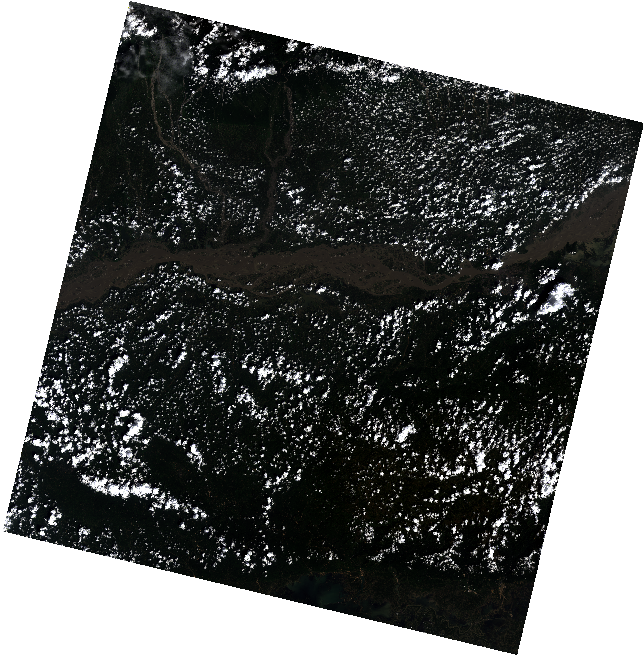
\includegraphics{images/gdal/rgb} \end{center}

\hypertarget{apply-histogram-stretch-and-color-correction}{%
\subsection{Apply Histogram Stretch and Color
Correction}\label{apply-histogram-stretch-and-color-correction}}

\begin{Shaded}
\begin{Highlighting}[]
\ExtensionTok{gdal_translate}\NormalTok{ -scale 0 0.3 0 255 -exponent 0.5 -ot Byte ^}
  \ExtensionTok{rgb.tif}\NormalTok{ rgb_stretch.tif}
\end{Highlighting}
\end{Shaded}

\begin{center}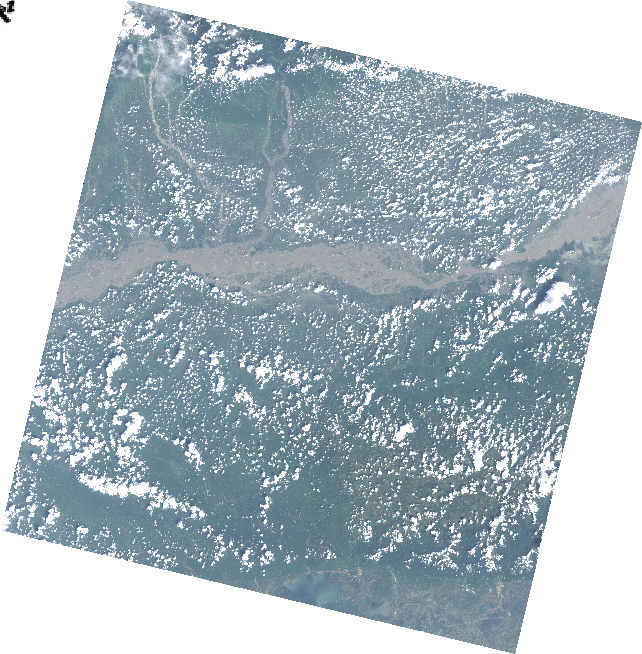
\includegraphics{images/gdal/rgb_stretch} \end{center}

\hypertarget{pan-sharpening}{%
\subsection{Pan Sharpening}\label{pan-sharpening}}

\begin{Shaded}
\begin{Highlighting}[]
\ExtensionTok{gdal_pansharpen}\NormalTok{ ^}
  \ExtensionTok{landsat8/RT_LC08_L1TP_137042_20190920_20190926_01_T1_2019-09-20_B8.TIF}\NormalTok{ ^}
  \ExtensionTok{rgb.tif}\NormalTok{ pansharpened.tif -r bilinear -co COMPRESS=DEFLATE -co PHOTOMETRIC=RGB}

\ExtensionTok{gdal_translate}\NormalTok{ -scale 0 0.3 0 255 -exponent 0.5 -ot Byte -a_nodata 0 ^}
  \ExtensionTok{pansharpened.tif}\NormalTok{ pansharpened_stretch.tif}
\end{Highlighting}
\end{Shaded}

\begin{center}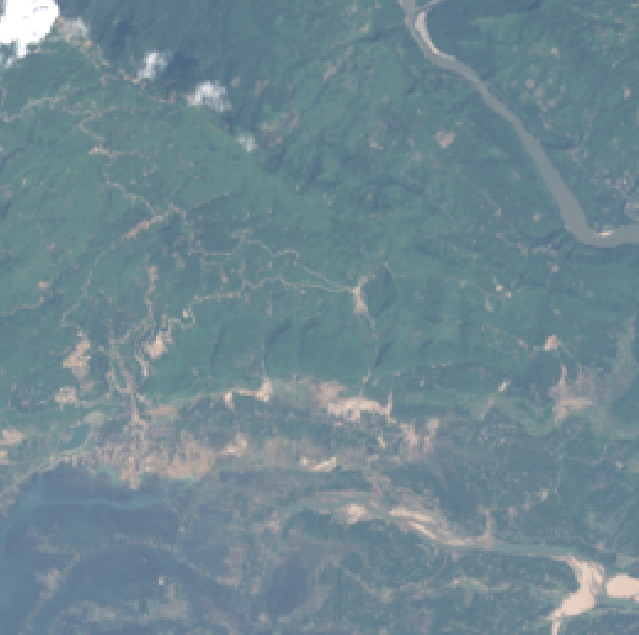
\includegraphics{images/gdal/pansharpen_before} \end{center}

\begin{center}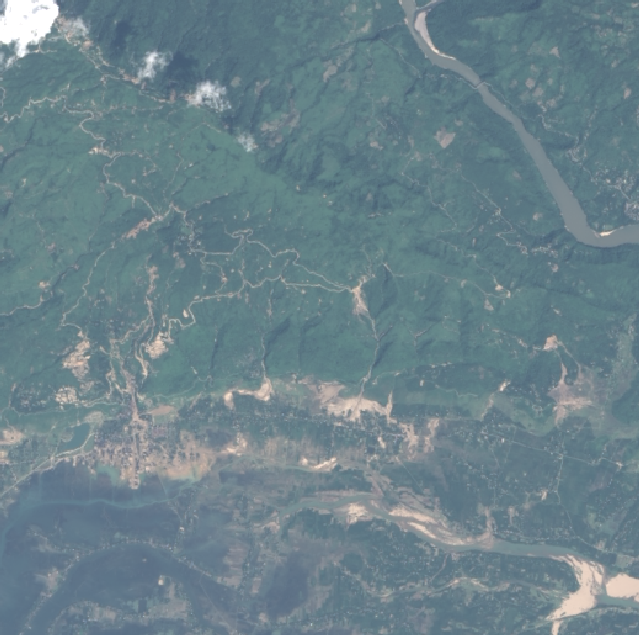
\includegraphics{images/gdal/pansharpen_after} \end{center}

\hypertarget{computing-ndvi}{%
\subsection{Computing NDVI}\label{computing-ndvi}}

\begin{Shaded}
\begin{Highlighting}[]
\ExtensionTok{gdalinfo}\NormalTok{ -stats ^}
  \ExtensionTok{landsat8/RT_LC08_L1TP_137042_20190920_20190926_01_T1_2019-09-20_B4.TIF}
\end{Highlighting}
\end{Shaded}

It is important to set nodata value. As seen from the output above,
nodata is set to -999.

\begin{Shaded}
\begin{Highlighting}[]
\ExtensionTok{gdal_calc}\NormalTok{ ^}
  \ExtensionTok{-A}\NormalTok{ landsat8/RT_LC08_L1TP_137042_20190920_20190926_01_T1_2019-09-20_B5.TIF ^}
  \ExtensionTok{-B}\NormalTok{ landsat8/RT_LC08_L1TP_137042_20190920_20190926_01_T1_2019-09-20_B4.TIF ^}
  \ExtensionTok{--outfile}\NormalTok{ ndvi.tif --calc=}\StringTok{"(A-B)/(A+B)"}\NormalTok{ --NoDataValue=-999}
\end{Highlighting}
\end{Shaded}

\begin{center}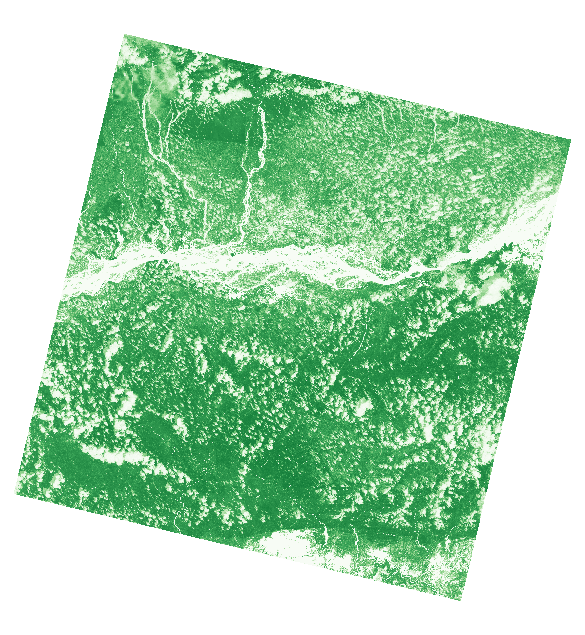
\includegraphics{images/gdal/ndvi} \end{center}

\hypertarget{georeferencing}{%
\section{Georeferencing}\label{georeferencing}}

\hypertarget{georeferencing-images-with-corner-coordinates}{%
\subsection{Georeferencing images with corner
coordinates}\label{georeferencing-images-with-corner-coordinates}}

You can easily assign bounding box coordinates to any image using the
\texttt{a\_ullr} option.

\begin{Shaded}
\begin{Highlighting}[]
\ExtensionTok{gdalinfo}\NormalTok{ earth_at_night.jpg}

\ExtensionTok{gdal_translate}\NormalTok{ -a_ullr -180 90 180 -90 -a_srs EPSG:4326 ^}
  \ExtensionTok{earth_at_night.jpg}\NormalTok{ earth_at_night.tif ^}
  \ExtensionTok{-co}\NormalTok{ PHOTOMETRIC=RGB -co COMPRESS=DEFLATE}

\ExtensionTok{gdalinfo}\NormalTok{ earth_at_night.tif}
\end{Highlighting}
\end{Shaded}

\begin{center}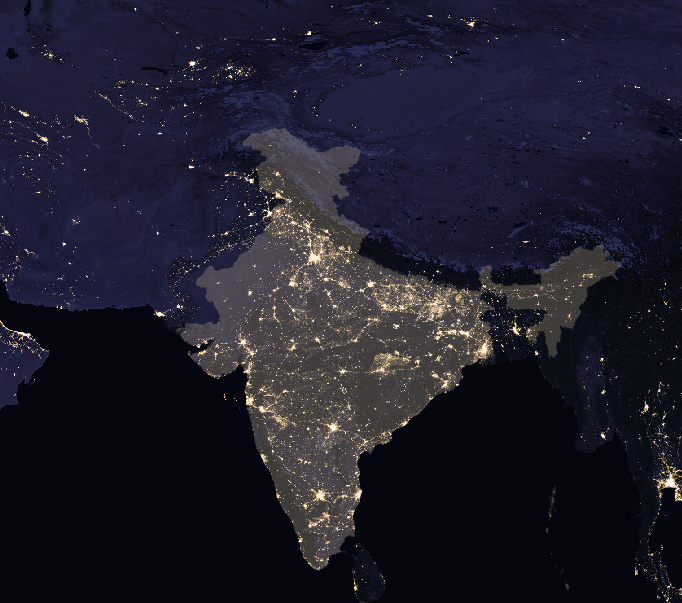
\includegraphics{images/gdal/earth_at_night} \end{center}

\hypertarget{georeferencing-with-gcps}{%
\subsection{Georeferencing with GCPs}\label{georeferencing-with-gcps}}

GCP format is {[}pixel line X Y{]}. You can use QGIS Georeferencer to
obtain the GCPs. Ideally, this process is used with images that have
known corner coordinates. In that case, if you know the image
dimensions, pixel and line values can be obtained easily.

Let's georeference this old scanned map.

\begin{center}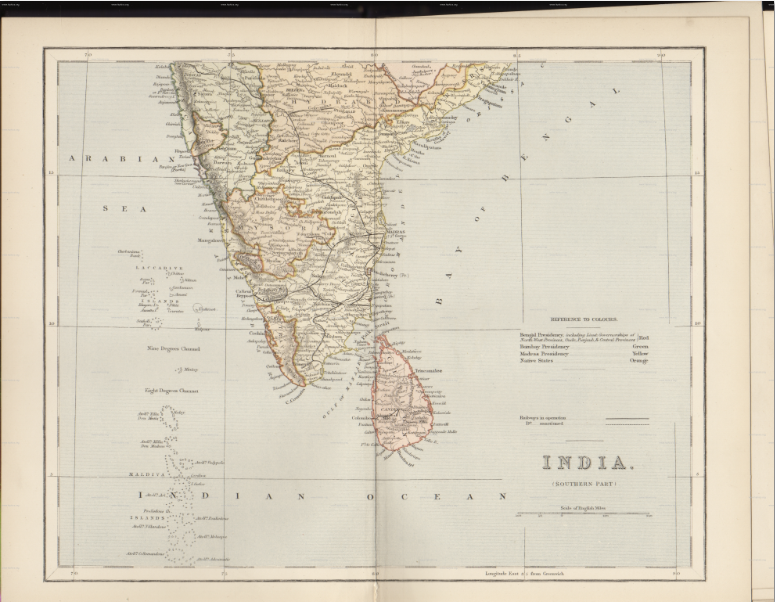
\includegraphics{images/gdal/scanned_map} \end{center}

First store the GCPs in the file

\begin{Shaded}
\begin{Highlighting}[]
\ExtensionTok{gdal_translate}\NormalTok{ ^}
  \ExtensionTok{-gcp}\NormalTok{ 418 893 70 15 ^}
  \ExtensionTok{-gcp}\NormalTok{ 380 2432 70 5 ^}
  \ExtensionTok{-gcp}\NormalTok{ 3453 2434  90 5 ^}
  \ExtensionTok{-gcp}\NormalTok{ 3407 895 90 15 ^}
  \ExtensionTok{-gcp}\NormalTok{ 2662 911 85 15 ^}
  \ExtensionTok{1870_southern-india.jpg}\NormalTok{ india-with-gcp.tif}
\end{Highlighting}
\end{Shaded}

Next, reproject the image using the GCPs

\begin{Shaded}
\begin{Highlighting}[]
\ExtensionTok{gdalwarp}\NormalTok{ -t_srs EPSG:4042 -r bilinear -tr 0.005 0.005 -overwrite ^}
  \ExtensionTok{india-with-gcp.tif}\NormalTok{ india-reprojected.tif}
\end{Highlighting}
\end{Shaded}

Try a Thin-plate-spline transformation with some compression options.

\begin{Shaded}
\begin{Highlighting}[]
\ExtensionTok{gdalwarp}\NormalTok{ -t_srs EPSG:4042 -tps -r bilinear -tr 0.005 0.005 -overwrite ^}
  \ExtensionTok{india-with-gcp.tif}\NormalTok{ india-reprojected.tif ^}
  \ExtensionTok{-co}\NormalTok{ COMPRESS=JPEG -co JPEG_QUALITY=50 -co PHOTOMETRIC=YCBCR}
\end{Highlighting}
\end{Shaded}

\begin{center}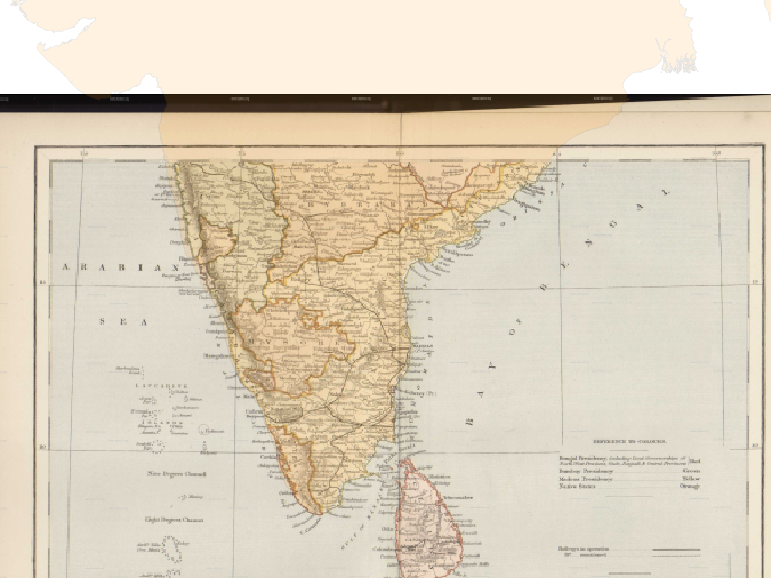
\includegraphics{images/gdal/georeference_gcp} \end{center}

\hypertarget{processing-of-aerial-imagery}{%
\section{Processing of Aerial
Imagery}\label{processing-of-aerial-imagery}}

\hypertarget{create-a-preview-image-from-source-tiles}{%
\subsection{Create a preview image from source
tiles}\label{create-a-preview-image-from-source-tiles}}

\begin{Shaded}
\begin{Highlighting}[]
\ExtensionTok{gdalbuildvrt}\NormalTok{ naip.vrt naip/*.jp2}
\ExtensionTok{gdal_translate}\NormalTok{ -of JPEG -outsize 2% 2% naip.vrt naip_preview.jpg }
\end{Highlighting}
\end{Shaded}

\begin{center}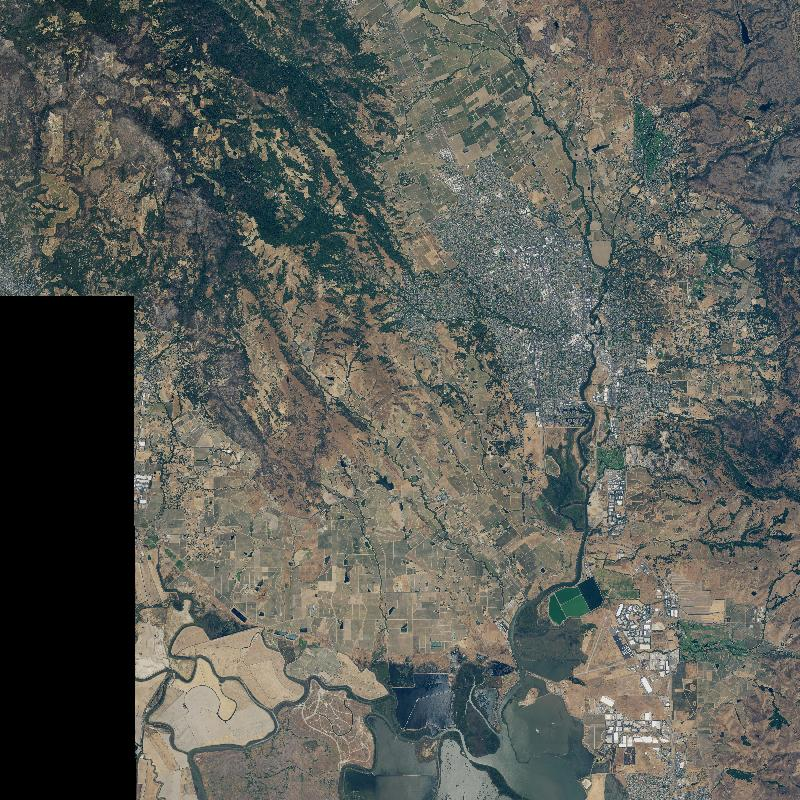
\includegraphics{images/gdal/naip_preview} \end{center}

\hypertarget{select-a-subset-of-tiles}{%
\subsection{Select a subset of tiles}\label{select-a-subset-of-tiles}}

\begin{Shaded}
\begin{Highlighting}[]
\ExtensionTok{gdaltindex}\NormalTok{ index.shp naip/*.jp2}
\end{Highlighting}
\end{Shaded}

We have the area of interest defined in the \texttt{aoi.shp} file. We
want to select and mosaic only the tiles intersecting our AOI

\begin{center}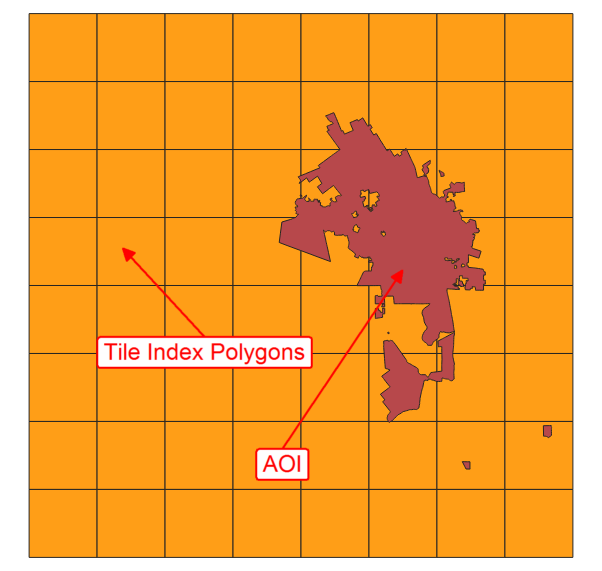
\includegraphics{images/gdal/aoiselection} \end{center}

Select and save the intersecting tiles using \emph{Extract by Location}
Processing algorithm in QGIS and save the selection as a CSV file
\texttt{selection.csv}.

\begin{center}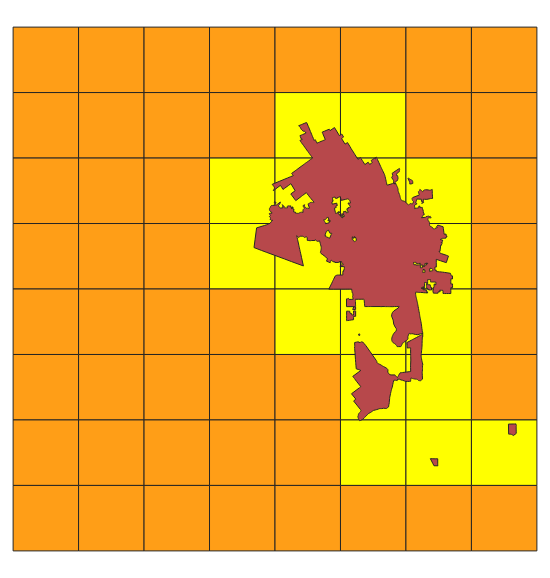
\includegraphics{images/gdal/aoiselected} \end{center}

Edit the file to remove the header line. This creates a text file with
source tile locations that can be supplied to the \texttt{gdalbuildvrt}
command.

\begin{Shaded}
\begin{Highlighting}[]
\ExtensionTok{gdalbuildvrt}\NormalTok{ -input_file_list selected.csv aoi.vrt}
\end{Highlighting}
\end{Shaded}

\hypertarget{mosaic-and-clip-to-aoi}{%
\subsection{Mosaic and clip to AOI}\label{mosaic-and-clip-to-aoi}}

\begin{Shaded}
\begin{Highlighting}[]
\ExtensionTok{gdalwarp}\NormalTok{ -cutline naip/aoi.shp  -crop_to_cutline aoi.vrt aoi.tif ^}
  \ExtensionTok{-co}\NormalTok{ PHOTOMETRIC=RGB -co COMPRESS=DEFLATE -dstnodata 0}
\end{Highlighting}
\end{Shaded}

\begin{center}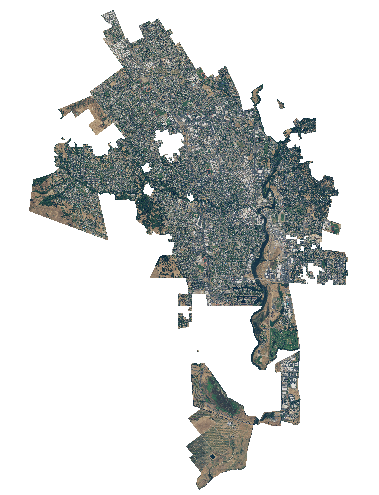
\includegraphics{images/gdal/mosaic} \end{center}

\hypertarget{multi-criteria-weighted-overlay-analysis}{%
\section{Multi Criteria Weighted Overlay
Analysis}\label{multi-criteria-weighted-overlay-analysis}}

Multi-criteria analysis is the process of the allocation of land to suit
a specific objective on the basis of a variety of attributes that the
selected areas should possess.

Although this is a common GIS operation, it is best performed in the
raster space. Below is the typical workflow to take source vector data,
transform them to appropriate rasters, re-classify them and perform
mathematical operations to do a suitability analysis.

The problem statement is \textbf{Locate the suitable areas for
development}, that are

\begin{itemize}
\tightlist
\item
  Close to roads
\item
  Away from waterbodies
\item
  Not in protected areas
\end{itemize}

\hypertarget{rasterize-vector-layers}{%
\subsection{Rasterize vector layers}\label{rasterize-vector-layers}}

For overlay analysis, all rasters must be of the same extent. So we
first find the extent of the dataset that we can use while rasterizing.

\begin{Shaded}
\begin{Highlighting}[]
\ExtensionTok{ogrinfo}\NormalTok{ -so osm/assam.gpkg boundary}
\end{Highlighting}
\end{Shaded}

\begin{Shaded}
\begin{Highlighting}[]
\ExtensionTok{gdal_rasterize}\NormalTok{ -ot Int16 -burn 1 -tr 15 15 -te 170134 2669018 798842 3097324 ^}
  \ExtensionTok{osm/assam.gpkg}\NormalTok{ -l roads roads.tif}
\end{Highlighting}
\end{Shaded}

\begin{center}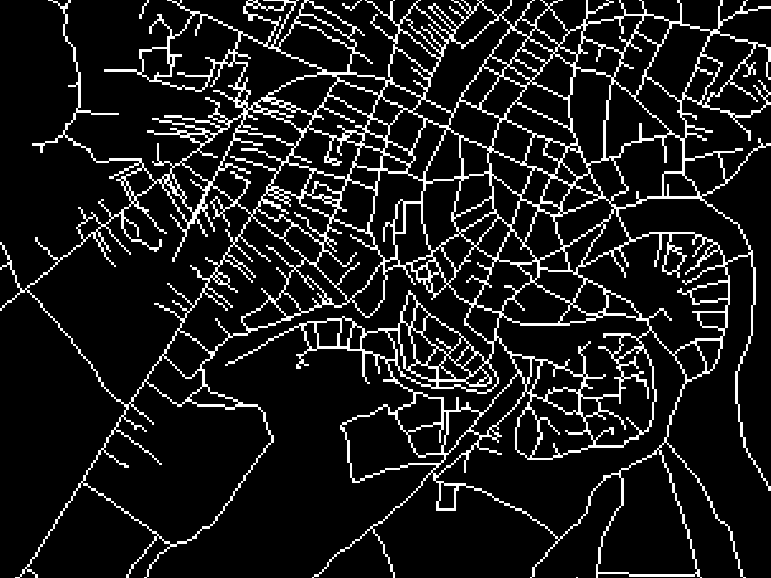
\includegraphics{images/gdal/roads_raster} \end{center}

\begin{Shaded}
\begin{Highlighting}[]
\ExtensionTok{gdal_rasterize}\NormalTok{ -ot Int16 -burn 1 -tr 15 15 -te 170134 2669018 798842 3097324 ^}
  \ExtensionTok{osm/assam.gpkg}\NormalTok{ -l boundary boundary.tif}
\end{Highlighting}
\end{Shaded}

Use \texttt{-i} for inverse rasterization. We want to rasterize
`un-protected' areas

\begin{Shaded}
\begin{Highlighting}[]
\ExtensionTok{gdal_rasterize}\NormalTok{ -i -ot Int16 -burn 1 -tr 15 15 -te 170134 2669018 798842 3097324 ^}
  \ExtensionTok{osm/assam.gpkg}\NormalTok{ -l protected_regions protected_regions.tif}
\end{Highlighting}
\end{Shaded}

We need a water layer, but the source data has a polygon and a polyline
water features layer. We create 2 rasters and then add them to create a
single water features raster.

\begin{Shaded}
\begin{Highlighting}[]
\ExtensionTok{gdal_rasterize}\NormalTok{ -ot Int16 -burn 1 -tr 15 15 -te 170134 2669018 798842 3097324 ^}
  \ExtensionTok{osm/assam.gpkg}\NormalTok{ -l water_polygons water_polygons.tif}

\ExtensionTok{gdal_rasterize}\NormalTok{ -ot Int16 -burn 1 -tr 15 15 -te 170134 2669018 798842 3097324 ^}
  \ExtensionTok{osm/assam.gpkg}\NormalTok{ -l water_polylines water_polylines.tif}


\ExtensionTok{gdal_calc}\NormalTok{ -A water_polygons.tif -B water_polylines.tif ^}
  \ExtensionTok{--outfile}\NormalTok{ water_add.tif --calc=}\StringTok{"A+B"}

\ExtensionTok{gdal_calc}\NormalTok{ -A water_add.tif --outfile water.tif ^}
  \ExtensionTok{--calc}\NormalTok{=}\StringTok{"A>0"}
\end{Highlighting}
\end{Shaded}

\begin{center}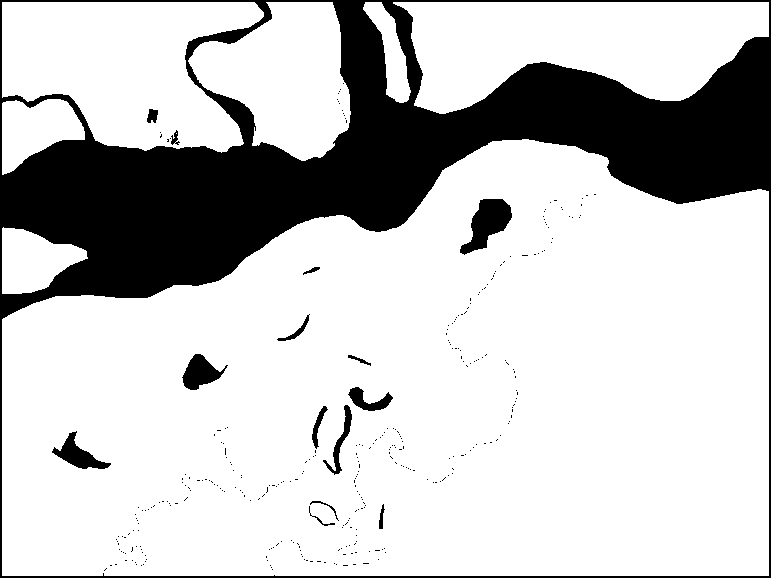
\includegraphics{images/gdal/water_raster} \end{center}

\hypertarget{generate-proximity-euclidean-distance-rasters}{%
\subsection{Generate proximity (Euclidean distance)
rasters}\label{generate-proximity-euclidean-distance-rasters}}

\begin{Shaded}
\begin{Highlighting}[]
\ExtensionTok{gdal_proximity}\NormalTok{ roads.tif roads_proximity.tif ^}
  \ExtensionTok{-ot}\NormalTok{ Int16 -distunits GEO}

\ExtensionTok{gdal_proximity}\NormalTok{ water.tif water_proximity.tif ^}
  \ExtensionTok{-ot}\NormalTok{ Int16 -distunits GEO}
\end{Highlighting}
\end{Shaded}

\begin{center}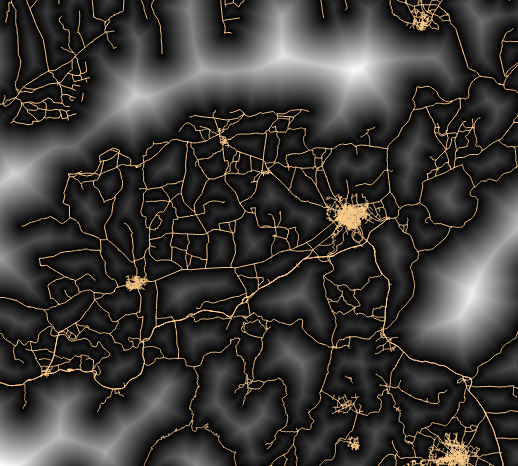
\includegraphics{images/gdal/roads_proximity} \end{center}

\hypertarget{re-classify-raster-values}{%
\subsection{Re-classify raster values}\label{re-classify-raster-values}}

\textbf{Roads} Give higher score to nearer pixels

0-1000m --\textgreater{} 100

1000-5000m --\textgreater{} 50

\textgreater5000m --\textgreater{} 10

\begin{Shaded}
\begin{Highlighting}[]
\ExtensionTok{gdal_calc}\NormalTok{ -A roads_proximity.tif --outfile roads_class.tif ^}
  \ExtensionTok{--calc}\NormalTok{=}\StringTok{"100*(A<=1000) + 50*(A>1000)*(A<=5000) + 10*(A>5000)"}
\end{Highlighting}
\end{Shaded}

\begin{center}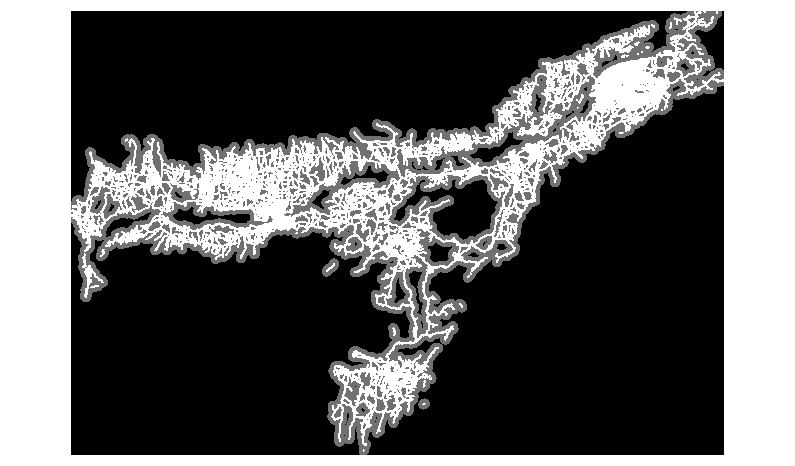
\includegraphics{images/gdal/roads_class} \end{center}

\textbf{Water} Give lower score to nearer pixels

0-1000m --\textgreater{} 10

1000 -5000m ---\textgreater{} 50

\textgreater5000m --\textgreater{} 100

\begin{Shaded}
\begin{Highlighting}[]
\ExtensionTok{gdal_calc}\NormalTok{ -A water_proximity.tif --outfile water_class.tif ^}
  \ExtensionTok{--calc}\NormalTok{=}\StringTok{"100*(A>5000) + 50*(A>1000)*(A<=5000) + 10*(A<1000)"}
\end{Highlighting}
\end{Shaded}

\begin{center}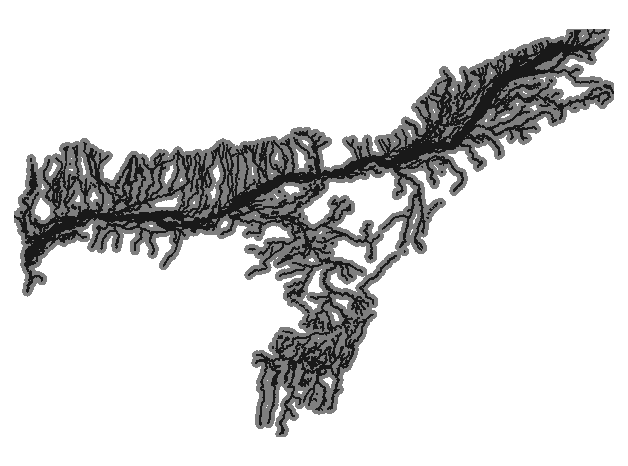
\includegraphics{images/gdal/water_class} \end{center}

\hypertarget{overlay-analysis}{%
\subsection{Overlay analysis}\label{overlay-analysis}}

Roads and Water have a range of values, but protected areas are either 0
or 1. So we combine these together accordingly.

\begin{Shaded}
\begin{Highlighting}[]
\ExtensionTok{gdal_calc}\NormalTok{ ^}
  \ExtensionTok{-A}\NormalTok{ roads_class.tif -B water_class.tif -C protected_regions.tif -D boundary.tif ^}
  \ExtensionTok{--outfile}\NormalTok{ suitability.tif --calc=}\StringTok{"(A + B)*(C>0)*D"}\NormalTok{ --NoDataValue=0}
\end{Highlighting}
\end{Shaded}

Smooth the output

\begin{Shaded}
\begin{Highlighting}[]
\ExtensionTok{gdalwarp}\NormalTok{ -r cubicspline -tr 60 60 -dstnodata 0 ^}
  \ExtensionTok{suitability.tif}\NormalTok{ suitability_final.tif}
\end{Highlighting}
\end{Shaded}

\begin{center}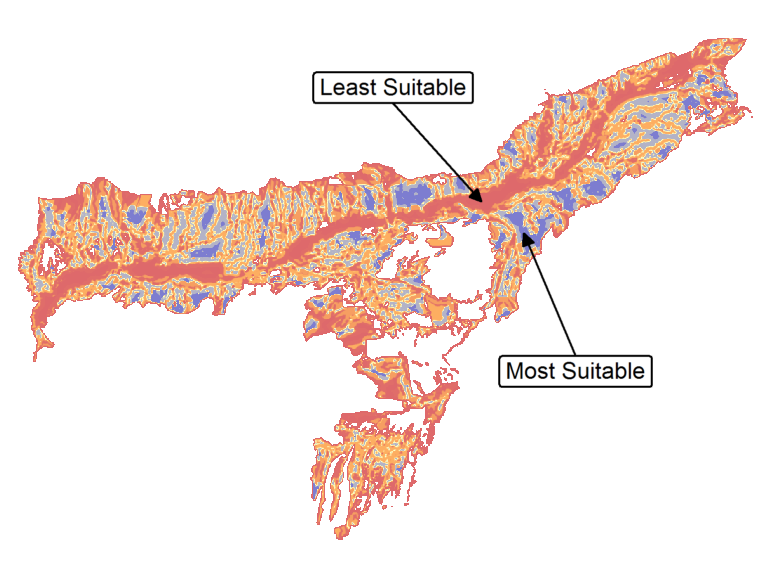
\includegraphics{images/gdal/suitability} \end{center}

\hypertarget{running-commands-in-batch}{%
\section{Running commands in batch}\label{running-commands-in-batch}}

You can run the GDAL/OGR commands in a loop using Python. Open OSGeo4W
Shell and type the following to set the correct system paths

\begin{Shaded}
\begin{Highlighting}[]
\ExtensionTok{py3_env}
\end{Highlighting}
\end{Shaded}

Say you want to convert the format of the images from JPEG200 to
GeoTiff. You would run a command such as below.

\begin{Shaded}
\begin{Highlighting}[]
\ExtensionTok{gdal_translate}\NormalTok{ -of GTiff -co COMPRESS=JPEG }\DataTypeTok{\{input\}} \DataTypeTok{\{output\}}
\end{Highlighting}
\end{Shaded}

But it would be a lot of manual effort if you want to run the commands
on hundreds of input files. Here's where a simple python script can help
you automate running the commands in a batch. The data directory
contains a file called \texttt{batch.py} with the following python code.

\begin{Shaded}
\begin{Highlighting}[]
\ImportTok{import}\NormalTok{ os}

\NormalTok{input_dir }\OperatorTok{=} \StringTok{'naip'}

\NormalTok{command }\OperatorTok{=} \StringTok{'gdal_translate -of GTiff -co COMPRESS=JPEG }\SpecialCharTok{\{input\}}\StringTok{ }\SpecialCharTok{\{output\}}\StringTok{'}
\ControlFlowTok{for} \BuiltInTok{file} \KeywordTok{in}\NormalTok{ os.listdir(input_dir):}
  \ControlFlowTok{if} \BuiltInTok{file}\NormalTok{.endswith(}\StringTok{'.jp2'}\NormalTok{):}
    \BuiltInTok{input} \OperatorTok{=}\NormalTok{ os.path.join(input_dir, }\BuiltInTok{file}\NormalTok{)}
\NormalTok{    filename }\OperatorTok{=}\NormalTok{ os.path.splitext(os.path.basename(}\BuiltInTok{file}\NormalTok{))[}\DecValTok{0}\NormalTok{]}
\NormalTok{    output }\OperatorTok{=}\NormalTok{  os.path.join(input_dir, filename }\OperatorTok{+} \StringTok{'.tif'}\NormalTok{)}
\NormalTok{    os.system(command.}\BuiltInTok{format}\NormalTok{(}\BuiltInTok{input}\OperatorTok{=}\BuiltInTok{input}\NormalTok{, output}\OperatorTok{=}\NormalTok{output))}
\end{Highlighting}
\end{Shaded}

In OsGeo4W shell, run the following command to start batch processing on
all tiles contained in the \texttt{naip/} directory.

\begin{Shaded}
\begin{Highlighting}[]
\ExtensionTok{python3}\NormalTok{ batch.py}
\end{Highlighting}
\end{Shaded}

The data directory also contains an example of running the batch
commands in parallel using python's built-in multiprocessing library. If
your system has multi-core CPU, running commands in parallel like this
on multiple threads can give you performance boost over running them in
series.

\begin{Shaded}
\begin{Highlighting}[]
\ImportTok{import}\NormalTok{ os}
\ImportTok{from}\NormalTok{ multiprocessing }\ImportTok{import}\NormalTok{ Pool}
\ImportTok{from}\NormalTok{ timeit }\ImportTok{import}\NormalTok{ default_timer }\ImportTok{as}\NormalTok{ timer}

\NormalTok{input_dir }\OperatorTok{=} \StringTok{'naip'}

\NormalTok{command }\OperatorTok{=} \StringTok{'gdal_translate -of GTiff -co COMPRESS=JPEG }\SpecialCharTok{\{input\}}\StringTok{ }\SpecialCharTok{\{output\}}\StringTok{'}

\KeywordTok{def}\NormalTok{ process(}\BuiltInTok{file}\NormalTok{):}
    \BuiltInTok{input} \OperatorTok{=}\NormalTok{ os.path.join(input_dir, }\BuiltInTok{file}\NormalTok{)}
\NormalTok{    filename }\OperatorTok{=}\NormalTok{ os.path.splitext(os.path.basename(}\BuiltInTok{file}\NormalTok{))[}\DecValTok{0}\NormalTok{]}
\NormalTok{    output }\OperatorTok{=}\NormalTok{  os.path.join(input_dir, filename }\OperatorTok{+} \StringTok{'.tif'}\NormalTok{)}
\NormalTok{    os.system(command.}\BuiltInTok{format}\NormalTok{(}\BuiltInTok{input}\OperatorTok{=}\BuiltInTok{input}\NormalTok{, output}\OperatorTok{=}\NormalTok{output))}
    
\NormalTok{files }\OperatorTok{=}\NormalTok{ [}\BuiltInTok{file} \ControlFlowTok{for} \BuiltInTok{file} \KeywordTok{in}\NormalTok{ os.listdir(input_dir) }\ControlFlowTok{if} \BuiltInTok{file}\NormalTok{.endswith(}\StringTok{'.jp2'}\NormalTok{)]}

\ControlFlowTok{if} \VariableTok{__name__} \OperatorTok{==} \StringTok{'__main__'}\NormalTok{:}
\NormalTok{  start }\OperatorTok{=}\NormalTok{ timer()}
\NormalTok{  p }\OperatorTok{=}\NormalTok{ Pool(}\DecValTok{4}\NormalTok{)}
\NormalTok{  p.}\BuiltInTok{map}\NormalTok{(process, files)}
\NormalTok{  end }\OperatorTok{=}\NormalTok{ timer()}
  \BuiltInTok{print}\NormalTok{(end }\OperatorTok{-}\NormalTok{ start)}
  
\NormalTok{  start }\OperatorTok{=}\NormalTok{ timer()}
  \ControlFlowTok{for} \BuiltInTok{file} \KeywordTok{in}\NormalTok{ files:}
\NormalTok{    process(}\BuiltInTok{file}\NormalTok{)}
\NormalTok{  end }\OperatorTok{=}\NormalTok{ timer()}
  \BuiltInTok{print}\NormalTok{(end }\OperatorTok{-}\NormalTok{ start)}
\end{Highlighting}
\end{Shaded}

The script runs the commands both in parallel and serial mode and prints
the time taken by each of them.

\begin{Shaded}
\begin{Highlighting}[]
\ExtensionTok{python3}\NormalTok{ batch-parallel.py}
\end{Highlighting}
\end{Shaded}

\hypertarget{data-credits}{%
\section{Data Credits}\label{data-credits}}

\begin{itemize}
\tightlist
\item
  OpenStreetMap (osm) data layers: Data/Maps Copyright 2019 Geofabrik
  GmbH and OpenStreetMap Contributors.
  \href{https://download.geofabrik.de/asia/india.html}{OSM India free
  extract} downloaded from Geofabrik.
\item
  Landsat: Landsat-8 image courtesy of the U.S. Geological Survey. Image
  downloaded from
  \href{https://console.cloud.google.com/marketplace/details/usgs-public-data/landast}{Google
  Cloud Platform} and pre-processed using
  \href{https://fromgistors.blogspot.com/p/semi-automatic-classification-plugin.html}{Semi
  Automatic Classification Plugin from QGIS}
\item
  Earth at Night image: Credit: NASA Earth Observatory/NOAA NGDC. Earth
  at Night flat hi-resolution map downloaded from
  \href{https://earthobservatory.nasa.gov/features/NightLights/page3.php}{NASA
  earth observatory}
\item
  William Mackenzie 1870 map of Southern India: out-of-copyright scanned
  map downloaded from
  \href{http://www.hipkiss.org/data/maps.html}{Hipkiss's Scanned Old
  Maps}
\item
  NAIP 2016 Aerial Imagery for California: The National Agriculture
  Imagery Program (NAIP). USDA-FSA-APFO Aerial Photography Field Office.
  Downloaded from
  \href{https://nrcs.app.box.com/v/naip/folder/18144379349}{NRCS}
\end{itemize}

\hypertarget{license}{%
\section{License}\label{license}}

This course is licensed under a
\href{http://creativecommons.org/licenses/by/4.0/deed.en_US}{Creative
Commons Attribution 4.0 International License}. You are free to use the
material in any form as you wish. Kindly give appropriate credit to the
original author.

© 2019 Ujaval Gandhi
\href{http://spatialthoughts.com}{www.spatialthoughts.com}


\end{document}
